\graphicspath{{chapters/images/0203/}}

\chapter{Statistical decision theory II}
  Just like in the regression setting, there are parametric and non-parametric
  methods in a classification setting too, these methods being:
  \begin{itemize}
    \item \textbf{Logistic regression} (parametric classification)
    \item \textbf{K nearest neighbour} (non-parametric classification)
  \end{itemize}

  \section{K nearest neighbour for classification}
    K-nearest neighbour is a non-parametric method for classification, meaning
    it allows to estimate the probability of a testing observation belonging to
    each of the classes. Formally this can be written as:

    $$P(Y = j | \vec{X} = \vec{x}_0), \; \text{ for } j = 1, \dots, C$$ 

    Where:
    \begin{itemize}
      \item $\vec{x}_0$ is the test observation
      \item $j$ is a specific class
      \item $C$ is the number of classes
    \end{itemize}
    
    \textbf{$K$} is a positive integer and represents the number of training
    data points closest to the observation data point to consider when
    classifying. $K$ is called \textbf{tuning parameter}, meaning that it can be
    tweaked in order to change how the model works; notice that the model is
    still non-parametric since $K$ does not depend on the training data points.

    In order to use this method you have to: 
    \begin{enumerate}
      \item \textbf{Identify the K training observations} that are closest
      (according to some distance, typically we consider the Eucledian distance)
      to $\vec{x}_0$. These observations  are then indexed with $\vec{N}_0$.

      \item \textbf{Compute the probability of the observation to belong to each
      of the classes} using the following formula:

      $$
      \hat{P(Y = j | \vec{X} = \vec{x}_0)} = \frac{1}{k}\sum_{i \in \vec{N}_0}{I(\hat{y_i} = j)},\;
      \text{ where } j = 1, \dots, C
      $$     

      Put into words, the equation above means: compute the probability that,
      given a test observation $\vec{x}_0$, it belongs to a specific class $j$
      by dividing the number of neighbours belonging to that class by the number
      of neighbours ($K$). The $I$ is an indicator variable that equals $1$ if
      $y_i \neq \hat{y_i}$, while instead it is equal to $0$ if $y_i =
      \hat{y_i}$. The indicator is used for each $i \in \vec{N_0}$ observation.
      Repeat for each class.
    \end{enumerate} 

\begin{figure}[H]
\caption{Classification process with K-neighbour method}
\centering
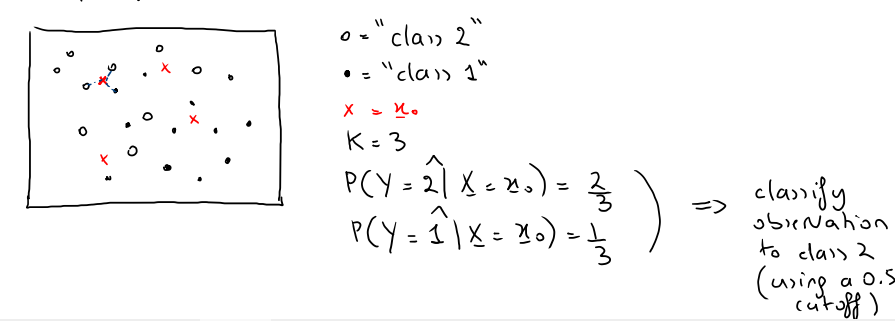
\includegraphics[width=0.6\textwidth]{Kneighbour}
\end{figure}



    \subsection{Bias-Variance trade off in K nearest neighbour classification}

    \begin{figure}[H]
      \caption{Tuning the $ K $ parameter}
      \centering
      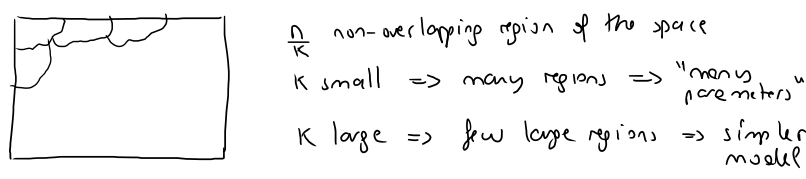
\includegraphics[width=0.6\textwidth]{KneigComplexityLogic}
      \label{KneigCompLog}
      \end{figure}

      The tuning parameter $K$ relates to the complexity of the model and it is
      the determinant to balance the bias and the variance of the model. Usually
      the value of $K$ is chosen using some training data. Intuitively (NOT
      formally), the model space could be considered as an area of dimension $n$
      which is divided in regions containing $k$ training points, therefore you
      have $\frac{n}{k}$ regions, hence:
      \begin{itemize}
        \item if \textbf{K is small}, then there are many small regions in the
        space and the model is complex. For this reason, if we change
        $\vec{x}_0$ with another value, the decision surface position changes
        quite a lot; if K is too small, the model could be overfitting and thus
        perform poorly with new test data points (low bias, high variance).
        \item if \textbf{K is large}, then there are few big regions in the
        space and the model is simple. For this reason, if we change $\vec{x}_0$
        with another value, the decision surface position will barely change; if
        K is too big, the model will give similar results for many different
        values of $\vec{x}_0$ (high bias, low variance).
      \end{itemize}


\begin{figure}[ht]
\caption{Complex and smooth decision surfaces, that respectively belong to complex models and simpler models}
\centering
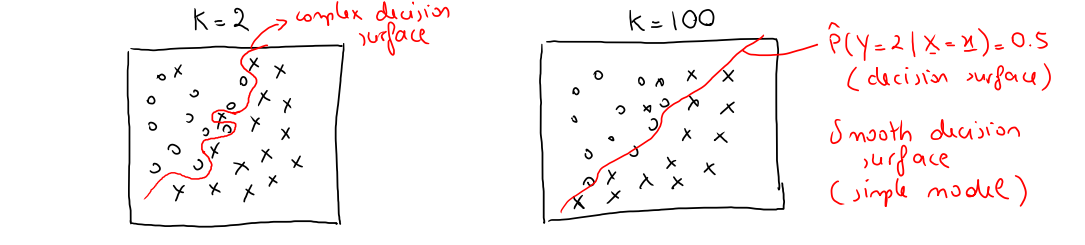
\includegraphics[width=0.95\textwidth]{KneighbourDecisionSurf}
\label{}
\end{figure}

\begin{figure}[ht]
\caption{Error rate on test data (red), error rate on training data (black), Bayes|constant error rate}
\centering
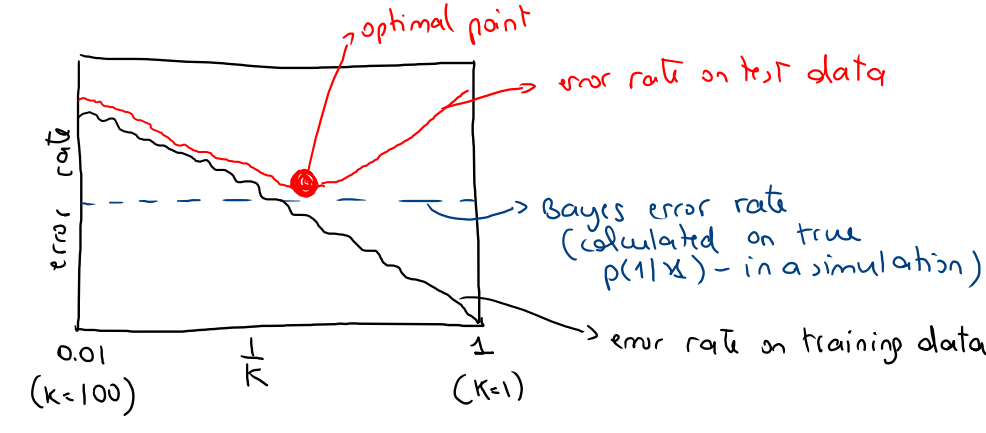
\includegraphics[width=0.8\textwidth]{KneighbourSimpleAgainstComplex}
\label{errorRate}
\end{figure}

The graph shown in figure \ref{errorRate} represents the behaviour of different
error rates (on test data, the constant error, and on training data) depending
on the complexity of the model. As it can be seen ... 

\begin{center}
\textit{An increase in model complexity is always associated with a lowering of
the error rate on the training data, while it is not generally associated with a
decrease of the error rate performed on the test data. The latter in fact
decreases until a certain moment, when it starts to increase making a U-shaped
curvature. The best case scenario would be the model where both the error rates
are at their minimum. }\end{center}


  \section{Logistic regression} \label{sect: logisticReg}
    \subsection{Why we cannot use linear regression in classification setting}
    \textbf{Example 1:} We want to predict the medical condition of a patient in
    the emergency room based on their symptoms. Assume that $Y$ takes only 3
    possible values:
    $$
    Y = \begin{cases}
          1 \text{ if stroke} \\
	      2 \text{ if overdose} \\
	      3 \text{ if seizures} \\
        \end{cases}
    $$

\begin{figure}[H]
\caption{Image representing a possible linear regression model for distinguishing classes}
\centering
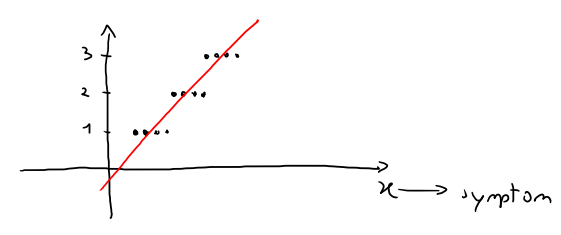
\includegraphics[width=0.6\textwidth]{LinearRegForClassification}
\label{}
\end{figure}


    A linear regression may seem to work, but you have some \textbf{problems}:
    \begin{itemize}
      \item If the order of the data points changes, the model changes.
      \item We are arbitrarely assigning an order to not necessarely ordered
      classes.
      \item We are imposing an arbitrary distance between the categories. 
    \end{itemize}

    \hfill

    \noindent\textbf{Example 2:} Assume that $Y$ from the previous example only
    takes 2 values:
    $$
    Y = \begin{cases}
          0 \text{ if stroke} \\
	        1 \text{ if overdose} \\
        \end{cases}
    $$
    In this case $Y$ is a random variable described by a Bernoulli distribution
    with some probability $p$ of taking the value 1, only two possible values
    are admitted; therefore 
    $$
    Y = \begin{cases}
          1 & p \\
	        0 & 1-p
        \end{cases}
    $$
    
    The Bernoulli random variable, that can assume either $0$ or $1$ value, has
    this particular expected value:
    
    \begin{align*}
      E[Y] = 0 \cdot (1-p) + 1 \cdot p = p && \text{where $p$ represents the probability of getting a $1$}
    \end{align*}
     
    Given these premises, you can write:
    $$E[Y|\vec{X} = \vec{x}] = p(1|\vec{x}) = \beta_0 + \beta_1 x_1 + \dots +
    \beta_px_p$$ Or considering just the Bernoulli case:
    $$\hat{E[Y|\vec{X} = \vec{x}]} = \hat{\beta}_0 + \hat{\beta}_1x_1$$ But
    notice that:
    \begin{itemize}
      \item $p(1|\vec{x}) \in (0, 1)$, so the probability should span between
      $0$ to $1$
      \item $\beta_0 + \beta_1 x_1 + \dots + \beta_px_p \in (-\infty, +\infty)$,
      yet using linear regression the probability spans over the entirety of
      $\mathbb{R}$.
    \end{itemize}
    
	Any time a straight line is fit to a binary response that is coded as $0$ or
    $1$, in principle we can always predict $p(1 | \vec{x}) < 0$ for some values
    of $X$ and $p(1 | \vec{x})) > 1$ for others. Therefore we must find a way to
    normalize the regression in the range $(0,1)$.
    
    \subsection{Characteristics of the logistic regression}
    We have to model $p(1 | \vec{x})$ using a function that gives outputs
    between $ 0 $ and $1$ for each value of $X$. \textbf{Logistic regression}
    solves the problem by utilizing a function of the probability
    $p(1|\vec{x})$, namely $g$, such that
    $$g(p(1|\vec{x})) = \beta_0 + \beta_1 x_1 + \dots + \beta_px_p =
    \vec{\beta}^t\vec{x}$$
    
    Logistic regression uses the \textbf{logistic function} (also named sigmoid
    function or activation function), which is defined as
    $$p(1|\vec{x}) = \frac{e^{\beta_0 + \beta_1 x_1 + \dots + \beta_p x_p}}
                          {1+e^{\beta_0 + \beta_1 x_1 + \dots + \beta_p x_p}}$$                          
               
\begin{figure}[ht]
\caption{Linear regression (left) \textbf{vs} Logistic regression (right) for
classification problems. Notice on the left the fact that values under $0$ for
certain values of $\vec{x}$ are possible.}
\centering
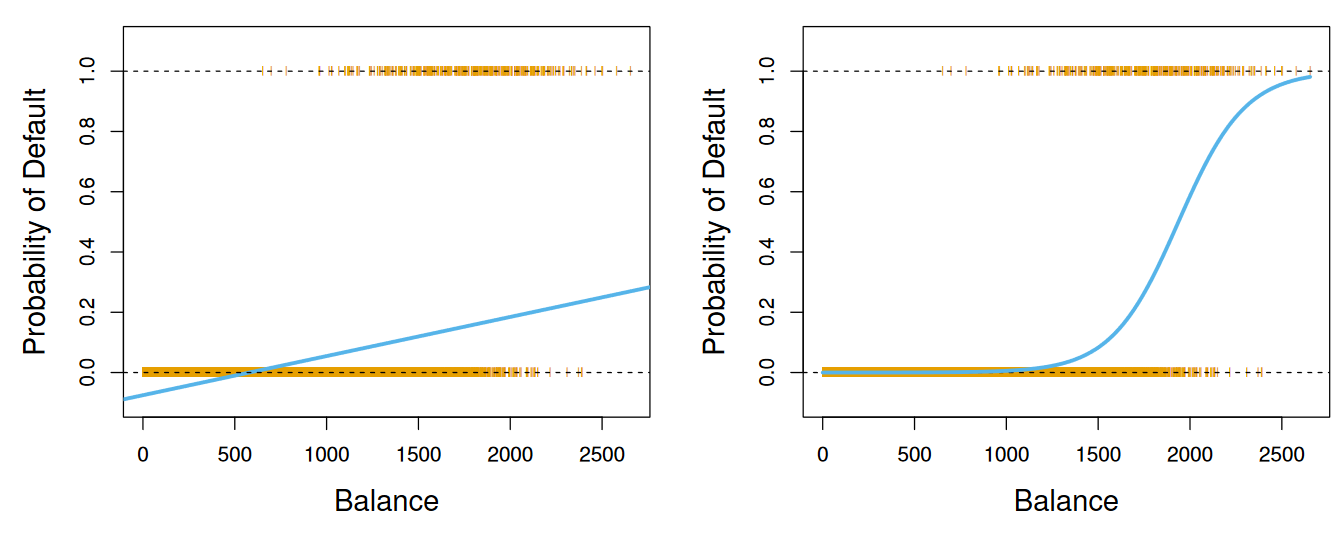
\includegraphics[width=0.85\textwidth]{LogisticReg}
\label{LogvsReg}
\end{figure}           
                          
    and it has the following properties (figure \ref{LogvsReg}):
    \begin{itemize}
      \item Its codomain corresponds to the interval $(0,1)$
      \item Taken any $ \vec{x} $, the logistic function classifies it to the
      "$1$" class if $p(1|\vec{x}) > 0.5$, otherwise to the "$0$" class.
    \end{itemize}

    \begin{figure}[ht]
      \caption{Linear regression (left) \textbf{vs} Logistic regression (right)
      for classification problems. Notice on the left the fact that values under
      $0$ for certain values of $\vec{x}$ are possible.}
      \centering
      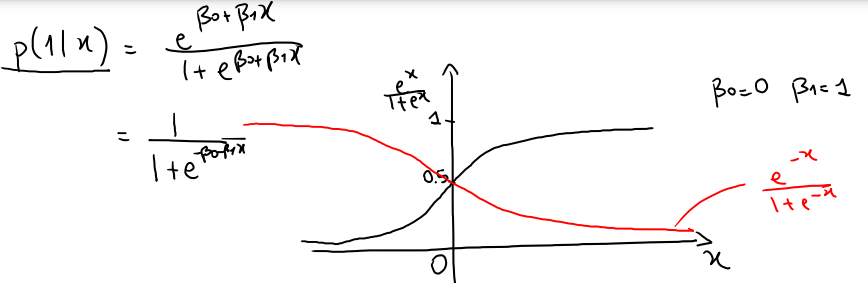
\includegraphics[width=0.7\textwidth]{logRegressionBernoulli}
      \label{classification: logRegExample}
      \end{figure}    

    Considering the \textbf{\textit{binomial}} case ($p(1|\vec{x}) =
    \frac{e^{\beta_0 + \beta_1 x_1}}{1+e^{\beta_0 + \beta_1 x_1}}$) with
    $\beta_0 = 0$ and $\beta_1 = 1$, as shown in figure \ref{classification:
    logRegExample}, the curve is sigmoid shape with intercept in $y=0.5$. It
    increases when the value of $\beta_1 > 0$.
    
    % The $g$ function is the inverse of the conversion from linear regression
    % to logistic function. %#TODO not so clear to me why this
    
    In the binomial case, the logistic function can be written as:
	\begin{align*}
	  p(1|\vec{x}) & = \frac{e^{\beta_0 + \beta_1 x_1}} {1+e^{\beta_0 + \beta_1 x_1}}
	               & \text{binomial case for simplicity} \\
	               & = \frac{e^{\beta_0 + \beta_1 x_1}} {e^0+e^{\beta_0 + \beta_1 x_1}}
	               & \text{reorganizing for clarity} \\
	               & = \frac{1}{e^{\beta_0 + \beta_1 x_1}} \cdot \frac{e^{\beta_0 + \beta_1 x_1}}{\frac{e^0}{e^{\beta_0 + \beta_1 x_1}} + 1}
	               & \text{by collecting } e^{\beta_0 + \beta_1 x_1} \text{ from the denominator}\\
	               & = \frac{1}{\frac{e^0}{e^{\beta_0 + \beta_1 x_1}} + 1} 
	               & \text{simplifying}\\ 
	               & = \frac{1}{1 + e^{-\beta_0 - \beta_1 x_1}}
	               & \text{since } \frac{a^x}{a^y} = a^{x-y}
	\end{align*}

	
    Let us define a quantity called \textbf{odds}, which is the ratio between
    positive and negative outcomes (the fraction of the probability of obtaining
    result $1$ over the one corresponding to the obtaining class $0$).

	\begin{align*}
	  \text{Odds } &= \frac{p(1|\vec{x})}{1 - p(1|\vec{x})}
	               & \text{by definition}\\
	               &= \frac{\frac{e^{\vec{\beta}^t\vec{x}}}{1 + e^{\vec{\beta}^t\vec{x}}}}
	                       {1 - \frac{e^{\vec{\beta}^t\vec{x}}}{1 + e^{\vec{\beta}^t\vec{x}}}}
	               & \text{since } p(1|\vec{x}) = \vec{\beta}^t\vec{x} \\
	               &= \frac{\frac{e^{\vec{\beta}^t\vec{x}}}{1 + e^{\vec{\beta}^t\vec{x}}}}
	                       {\frac{1 + e^{\vec{\beta}^t\vec{x}} - e^{\vec{\beta}^t\vec{x}}}{1 + e^{\vec{\beta}^t\vec{x}}}}
	               & \text{minimum common denominator}\\
	               &= \frac{\frac{e^{\vec{\beta}^t\vec{x}}}{1 + e^{\vec{\beta}^t\vec{x}}}}
	                       {\frac{1}{1 + e^{\vec{\beta}^t\vec{x}}}}
	               & \text{simplifying}\\
	               &= \frac{e^{\vec{\beta}^t\vec{x}}}{1 + e^{\vec{\beta}^t\vec{x}}} \cdot
	                       \frac{1 + e^{\vec{\beta}^t\vec{x}}}{1}
	               & \text{reorganizing}\\
	               &= e^{\vec{\beta}^t\vec{x}}
	               & \text{simplifying}\\
	\end{align*}
    
	As it can be seen from the formula, $\text{Odds} = \frac{p(1|\vec{x})}{1 -
p(1|\vec{x})} = e^{\vec{\beta}^t\vec{x}} $ can take any value between $[0,
+\inf]$, indicating very low and high probabilities of positive outcome
respectively (the bigger is the value of $p(1|\vec{x})$, the lower is the value
of $1- p(1|\vec{x})$). \\

\noindent \textbf{Example}: on average $1$ in $5$ people with an odds of
$\frac{1}{4}$ will default, since $p(X) = 0.2$ implies an odds of
$\frac{0.2}{1-0.2} = \frac{1}{4}$. \\

The predictor for this measure is called \textbf{log-odds} or \textbf{logit} and
it is obtained applying a logarithmic tranformation, hence:
    $$
    \log\left(\frac{p(1|\vec{x})}{1 - p(1|\vec{x})}\right) 
    = \beta_0 + \beta_1 x_1 + \dots + \beta_px_p 
    = \vec{\beta}^t\vec{x}
    $$
    % TODO Add image of logit
    
    The logistic regression model (assuming the random variable to be Bernoulli
    distributed \textbf{[}$Y|\vec{X} = \vec{x} \sim
    Bernoulli(p(1|\vec{x}))$\textbf{]}) is defined as follows:

    $$\log\left(\frac{p(1|\vec{x})}{1 - p(1|\vec{x})}\right) = \beta_0 + \beta_1
    x_1 + \dots + \beta_px_p $$
    
    The coefficients can be interpeted as follows: a one-unit increase in $x_j$
    (while everithing else is kept constant) induces a change in the log-odds of
    $\beta_j$, while instead it multiplies the odds by $e^{\beta_j}$ (see the
    example written below). \\

    \noindent\textbf{Example}: Logistic regression for a single predictor $X$
    which is binary.

    \begin{figure}[ht]
      \caption{Demonstration written by the professor}
      \centering
      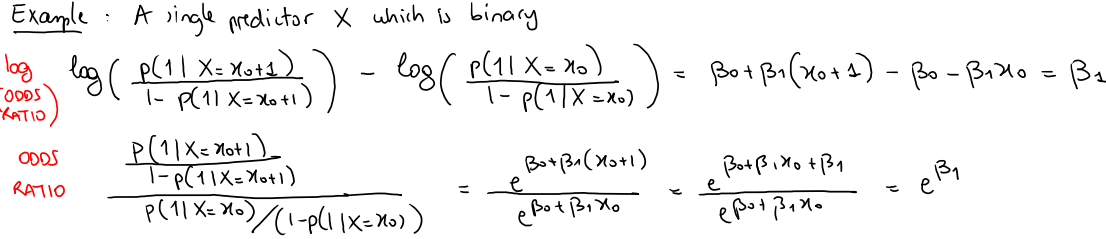
\includegraphics[width=0.85\textwidth]{demonstrationLogoddsChange}
      \label{logoddchange}
      \end{figure}

    To compute the change of the log-odds for a one-unit change of $X$ we
    compute
    \begin{align*}
    \log(\text{odds ratio})
      & = \log\left(\frac{p(1|X=x_1+1)}{1-p(1|X=x_1+1)}\right)-\log\left(\frac{p(1|X=x_1)}{1-p(1|X=x_1)}\right)
      & \text{log odds in 1 minus log odds in 0}\\
      & = \beta_0 + \beta_1 (x_1 + 1) - \beta_0 - \beta_1x_1 
      & \text{by definition of logistic regression}\\
      & = \beta_1
      & \text{simplifying}
\end{align*}
 
    This quantity is called \textbf{log(odds ratio)} since the subtraction of
    two logarithms in the same base is equal to the logarithm of the ratio of
    the arguments. Notice that, as expected, a one unit increase of the value of
    $x_1$ results in an increment of \textbf{$\beta_1$}.

    If we instead consider the same increment for the \textbf{odds ratio}, we
    get:

    \begin{align*}
      \text{odds ratio}
      & = \frac{\frac{p(1|X=x_0+1)}{1-p(1|X=x_0+1)}}{\frac{p(1|X=x_0)}{1-p(1|X=x_0)}} 
      & \text{odds in 1 divided by odds in 0}\\
      & = \frac{e^{\beta_0 + \beta_1 (x_0 + 1)}}{e^{\beta_0 + \beta_1 x_0}}
      & \text{using the fact that } \log\left(\frac{p(1|\vec{x})}{1 - p(1|\vec{x})}\right)= \vec{\beta}^t\vec{x}\\
      & = \frac{e^{\beta_0 + \beta_1x_0 + \beta_1}}{e^{\beta_0 + \beta_1 x_0}} 
      & \text{rearranging}\\
      & = e^{\beta_1}
      & \text{since } \frac{x^a}{x^b} = x^{a-b}
    \end{align*}
    Therefore we have an increase of \textbf{$e^{\beta_1}$} as expected.

    \subsection{Parameter estimation in logistic regression}
    When estimating parameters for non-linear regressions you often get
    non-closed form expressions, therefore the maximum likelihood(s) for the
    parameter(s) must be maximised numerically. Notice that, contrarily to
    linear regression, you cannot use the least square method. \\

    For instance, give some training data $(\vec{x}_i, y_i), \; i=1, \dots, n$,
    we want to estimate the best values of $\beta_0, \beta_1, \dots, \beta_p$ to
    fit the values of $y$. To do so we need to compute the maximum likelihood
    given that $Y$ is binary, thus
    $$Y|\vec{X} = \vec{x} \sim Bernoulli(p(1|\vec{x})), \; f(y|\vec{x}) =
    p(1|\vec{x})^y(1-p(1|\vec{x}))^{1-y}$$

    To put into words what is written here, for dummies like me, the probability
    that a point, obtained given some $\vec{x}$, is classified to the $0$ class,
    is equal to $p(1|\vec{x})^0 (1-p(1|\vec{x}))^{1-0} = 1 * (1-p(1|\vec{x}))$.
    Coherently, the probability that a point is classified to the $1$ class, is
    equal to $p(1|\vec{x})^1 (1-p(1|\vec{x}))^{1-1} = p(1|\vec{x}) * 1$. The
    probabilities of all the points are multiplied to obtain the likelihood
    function, written below:
    
    \begin{align*}
    L(\vec{\beta}) = \prod_{i=1}^{n}f(y_i|\vec{x}_i) = \prod_{i=1}^{n}p(1|\vec{x}_i)^{y_i}(1-p(1|\vec{x}_i))^{1-y_i} && \text{given some values of $\beta_0$ and $\beta_1$}
    \end{align*} %coul dbe n-y_i???
    
    We then compute the log-likelihood and reorganize it in order to make
    evident its dependence from $\vec{\beta}$:
    
    \begin{align*}
    l(\vec{\beta}) 
    &=\sum_{i=1}^{n}[y_i\log(p(1|\vec{x}_i))+(1-y_i)\log(1-p(1|\vec{x}_i))]
    & \text{applying logarithm}\\
    &=\sum_{i=1}^{n}\left[y_i\log(p(1|\vec{x}_i)) - y_i\log(1-p(1|\vec{x}_i)) +\log(1-p(1|\vec{x}_i))\right]
    & \text{multiplying}\\
    &=\sum_{i=1}^{n}\left[y_i\log\left(\frac{p(1|\vec{x}_i))}{1-p(1|\vec{x}_i))}\right)+\log(1-p(1|\vec{x}_i))\right]
    & \log(a) - \log(b) = \log\left(\frac{a}{b}\right)\\
    & \text{ but since } \log\left(\frac{p(1|\vec{x})}{1 - p(1|\vec{x})}\right)= \vec{\beta}^t\vec{x} \text{ and } 
      p(1|\vec{x}) = \frac{e^{\beta_0 + \beta_1 x_1}} {1+e^{\beta_0 + \beta_1 x_1}} &\\
    &=\sum_{i=1}^{n}\left[y_i\vec{\beta}^t\vec{x}_i+\log\left(1-\frac{e^{\vec{\beta}^t\vec{x}_i}}{1+e^{\vec{\beta}^t\vec{x}_i}  }\right)\right] &\\
    &=\sum_{i=1}^{n}\left[y_i\vec{\beta}^t\vec{x}_i+\log\left(\frac{1}{1+e^{\vec{\beta}^t\vec{x}_i}}\right)\right]
    & \text{using mcm and simplifying}\\
    &=\sum_{i=1}^{n}\left[y_i\vec{\beta}^t\vec{x}_i+\log(1)-\log\left(1+e^{\vec{\beta}^t\vec{x}_i}\right)\right]
    & \text{dividing the logarithms}\\
    & =\sum_{i=1}^{n}\left[y_i\vec{\beta}^t\vec{x}_i-\log\left(1+e^{\vec{\beta}^t\vec{x}_i}\right)\right]
    & \text{since }\log{((1)} = 0
    \end{align*}

    We then compute the first derivative in $\vec{\beta}$ (notice that since you
    want to derive in a vector, you need to take the partial derivatives in each
    of the elements of the vector):
    \begin{align*}
    \frac{\partial l(\beta)}{\partial \beta_j}
    &=\frac{\partial}{\partial \beta_j}\left(\sum_{i=1}^{n}\left[y_i\vec{\beta}^t\vec{x}_i-\log\left(1+e^{\vec{\beta}^t\vec{x}_i}\right)\right]\right) \; j = 0,\,\dots,\,p \\
    & \text{ but } \frac{\partial\vec{\beta}^t\vec{x}}{\partial\beta_j} 
      = \frac{\partial}{\partial\beta_j}(\beta_0 x_{i0} + \dots +\beta_p x_{ip}) = x_{ij} \text{ since the other terms simplify, consequently}\\
    &= \sum_{i=1}^{n}\left[y_ix_{ij}-\frac{1}{1+e^{\vec{\beta}^t\vec{x}_i}} * e^{\vec{\beta}^t\vec{x}_i} * x_{ij}\right] = 
    \sum_{i=1}^{n}\left[y_ix_{ij}-\frac{e^{\vec{\beta}^t\vec{x}_i}}{1+e^{\vec{\beta}^t\vec{x}_i}}x_{ij}\right] \\
    & \text{ but } \frac{e^{\vec{\beta}^{t}\vec{x}_i}} {1+e^{\vec{\beta}^{t}\vec{x}_i}} = p(1|\vec{x}) \text{ therefore} \\
    &=\sum_{i=1}^{n}\left[y_ix_{ij}-p(1|\vec{x}_i)x_{ij}\right]
    \end{align*}
    
    By setting this derivative to zero you obtain $p+1$ equations in $p+1$
    parameters (where $p$ is the number of $\beta$ parameters), therefore to optimize
    numerically the function (by solving the equations) you must use an
    optimization method like \textbf{Newton-Raphson}. The \textit{gml} function
    in R uses an iterative reweighted least-squares algorithm, which is a
    variation of the Newton-Raphson method. \\

    %Maybe it could be studied more the Newton_Raphson method, or study better
    %the way the function gml works in R #TODO

    From the optimization you get $\hat{\vec{\beta}} = \hat{\beta}_0,
    \hat{\beta}_1, \dots, \hat{\beta}_p $, which can be used to estimate
    $p(1|\vec{x})$, since
    $$\hat{p(1|\vec{x})} =
    \frac{e^{\hat{\vec{\beta}^t}\vec{x}}}{1+e^{\hat{\vec{\beta}^t}\vec{x}}}$$\\

    Look to pages $137-139$ from "\textit{An introduction to statistical learning with
    applications in R}" (doi:$10.1080/24754269.2021.1980261$) for examples.
